% Bengali report for PGBM Initial Solution V2.1.
\documentclass[10pt,a4paper]{article}
\usepackage{fontspec}
\usepackage{polyglossia}
\setmainlanguage{bengali}
\setotherlanguage{english}
\setmainfont[Script=Bengali]{Kohinoor Bangla}
\setsansfont[Script=Bengali]{Kohinoor Bangla}
\newfontfamily\bengalifonttt[Script=Bengali]{Kohinoor Bangla}
\newfontfamily\englishfont{Avenir Next}
\usepackage[a4paper,margin=20mm,headheight=24pt]{geometry}
\usepackage{amsmath,array,booktabs,enumitem,fancyhdr,float,graphicx,longtable,pdflscape,titlesec,xcolor,hyperref}
\definecolor{navy}{HTML}{17365D}
\definecolor{bluegray}{HTML}{EAF1F8}
\definecolor{midgray}{HTML}{5B6573}
\definecolor{rulegray}{HTML}{C9D1D9}
\hypersetup{colorlinks=true,linkcolor=navy,urlcolor=navy,pdftitle={PGBM Initial Solution V2.1 Cache Aware Recourse Report},pdfauthor={PGBM Thesis Simulation Work}}
\setlist[itemize]{label={-},leftmargin=*,itemsep=1pt,topsep=2pt}
\setlist[enumerate]{leftmargin=*,itemsep=3pt,topsep=2pt}
\titleformat{\section}{\Large\bfseries}{\thesection}{0.75em}{}
\titlespacing*{\section}{0pt}{2.5ex plus 0.4ex minus 0.2ex}{1ex plus 0.2ex}
\setlength{\parindent}{0pt}
\setlength{\parskip}{4pt}
\setlength{\emergencystretch}{2em}
\pagestyle{fancy}
\fancyhf{}
\fancyhead[L]{\textcolor{midgray}{PGBM Thesis Simulation}}
\fancyhead[R]{\textcolor{midgray}{Initial Solution V2.1}}
\fancyfoot[C]{\textcolor{midgray}{\thepage}}
\renewcommand{\headrulewidth}{0.4pt}
\renewcommand{\headrule}{\hbox to\headwidth{\color{rulegray}\leaders\hrule height \headrulewidth\hfill}}
\begin{document}
\begin{titlepage}
\thispagestyle{empty}
\vspace*{18mm}
{\color{navy}\rule{\textwidth}{1.5pt}}\\[10mm]
{\color{navy}\englishfont\bfseries\fontsize{25}{32}\selectfont Initial Solution V2.1\\Cache Aware Recourse Report\par}
\vspace{6mm}
{\color{midgray}\sffamily\Large One slot reserve parcel, paired experiment এবং ফলাফল\par}
\vfill
\begin{tabular}{@{}ll@{}}
\textbf{Project:} & PGBM thesis and simulation work\\
\textbf{সমাধানের ধরন:} & Cache aware one slot recourse\\
\textbf{Environment:} & Synthetic এবং DU outdoor\\
\textbf{মোট configuration:} & ২৪০টি paired configuration, ৭২০টি metrics row\\
\textbf{Seed:} & ১০১--১১০\\
\textbf{Report date:} & ৭ অক্টোবর ২০২৬
\end{tabular}
\vfill
\begin{center}
\colorbox{bluegray}{\begin{minipage}{0.88\textwidth}
এই report-এ V2.1 cache loading rule, feasibility guard, paired V2 control, cache hit evidence এবং one slot policy decision একই flow-তে ব্যাখ্যা করা হয়েছে।
\end{minipage}}
\end{center}
\vspace{12mm}
{\color{navy}\rule{\textwidth}{1.5pt}}
\end{titlepage}
\tableofcontents
\clearpage
\section{V2.1-এর core feature}
V2.1 হলো V2-এর উপর নির্মিত bounded cache aware recourse layer। Ordinary V2 mission route তৈরি হওয়ার পরে dispatch time-এ সর্বোচ্চ একটি reserve parcel load করা হয়। Payload slot, payload mass, full route energy, reserve energy, return route এবং ১২০ মিনিটের horizon feasible হলেই reserve load হয়। Reserve future undetected task দেখে নির্বাচন করা হয় না এবং flight-এর মাঝখানে reload করা হয় না। পরবর্তী replacement V2-এর one-for-one positive service-value gain rule অনুসরণ করে।
\begin{itemize}
\item At most one reserve parcel: একটি mission-এ সর্বোচ্চ একটি cache slot।
\item Feasibility guards: payload, mass, energy reserve, return এবং horizon।
\item Configured prior: default uniform prior এবং labelled water-heavy sensitivity prior।
\item Cache evidence: load, use, match, accepted hit, miss এবং returned parcel আলাদা record।
\item V2 isolation: canonical V1 এবং V2 code path ও evidence overwrite করা হয়নি।
\end{itemize}
\section{Experiment-এর সংক্ষিপ্ত চিত্র}
V2 control এবং প্রতিটি V2.1 policy একই seeded scenario-তে চালানো হয়েছে। দুইটি environment, ৩০/৬০/৯০ task load, ৩/৫/৮/১০ UAV এবং ১০টি seed ব্যবহার করে ২৪০টি scenario, ৭২০টি metrics row এবং ২৪০টি decision trace তৈরি হয়েছে। Matrix generation-এর জন্য bounded planner settings manifest-এ সংরক্ষিত আছে।
\section{Cache loading এবং recourse flow}
প্রথমে ordinary V2 route calculate হয়। এরপর configured prior থেকে একটি item নির্বাচন করা হয়। Free payload slot, remaining mass, cache সহ full route energy, reserve margin, return time এবং horizon check করা হয়। সব guard pass করলে reserve inventory mission state-এ রাখা হয়। Later replacement-এ cache বা released displaced inventory candidate demand satisfy করতে পারে, কিন্তু candidate শুধুমাত্র feasible positive service-value gain হলে accepted hit হয়। Loaded কিন্তু unused parcel mission শেষে returned হিসেবে record হয়।
\section{Aggregate performance}
\begin{table}[htbp]\centering\scriptsize
\caption{V2 control এবং V2.1 policy aggregate result।}
\begin{tabular}{@{}lrrrrrr@{}}\toprule
Variant & Episodes & Objective & Served & Delivery & Energy & Delay\\\midrule
V2 control & 240 & 17.01 ± 9.36 & 27.39 ± 15.40 & 48.2\% & 5613.94 ± 2225.71 & 18.23 ± 4.68 \\
Uniform cache & 240 & 17.25 ± 9.45 & 27.68 ± 15.65 & 49.0\% & 5679.48 ± 2244.19 & 17.86 ± 4.54 \\
Water heavy sensitivity & 240 & 17.34 ± 9.44 & 27.84 ± 15.52 & 49.2\% & 5704.77 ± 2264.83 & 18.07 ± 4.55 \\
\bottomrule\end{tabular}\end{table}
\section{Paired core findings}
প্রতিটি V2.1 row একই environment, task load, UAV count এবং seed-এর V2 control row-এর সঙ্গে তুলনা করা হয়েছে।
\begin{table}[htbp]\centering\scriptsize
\caption{V2.1 minus V2 paired delta।}
\begin{tabular}{@{}lrrrrrr@{}}\toprule
Variant & Episodes & $\Delta$ Objective & $\Delta$ Served & $\Delta$ Deferred & $\Delta$ Delay & $\Delta$ Energy\\\midrule
Uniform cache & 240 & 0.238 & 0.287 & -0.287 & -0.376 & 65.541 \\
Water heavy sensitivity & 240 & 0.328 & 0.454 & -0.454 & -0.163 & 90.831 \\
\bottomrule\end{tabular}\end{table}
দুইটি one-slot policy-তেই objective সামান্য বেড়েছে। Uniform policy-তে mean objective gain 0.238 এবং served task gain 0.288। Water-heavy sensitivity-তে gain 0.328 এবং 0.454। তবে reserve load-এর বড় অংশ unused অবস্থায় return করেছে এবং water-heavy policy-তে cache energy overhead বেশি।
\begin{figure}[htbp]\centering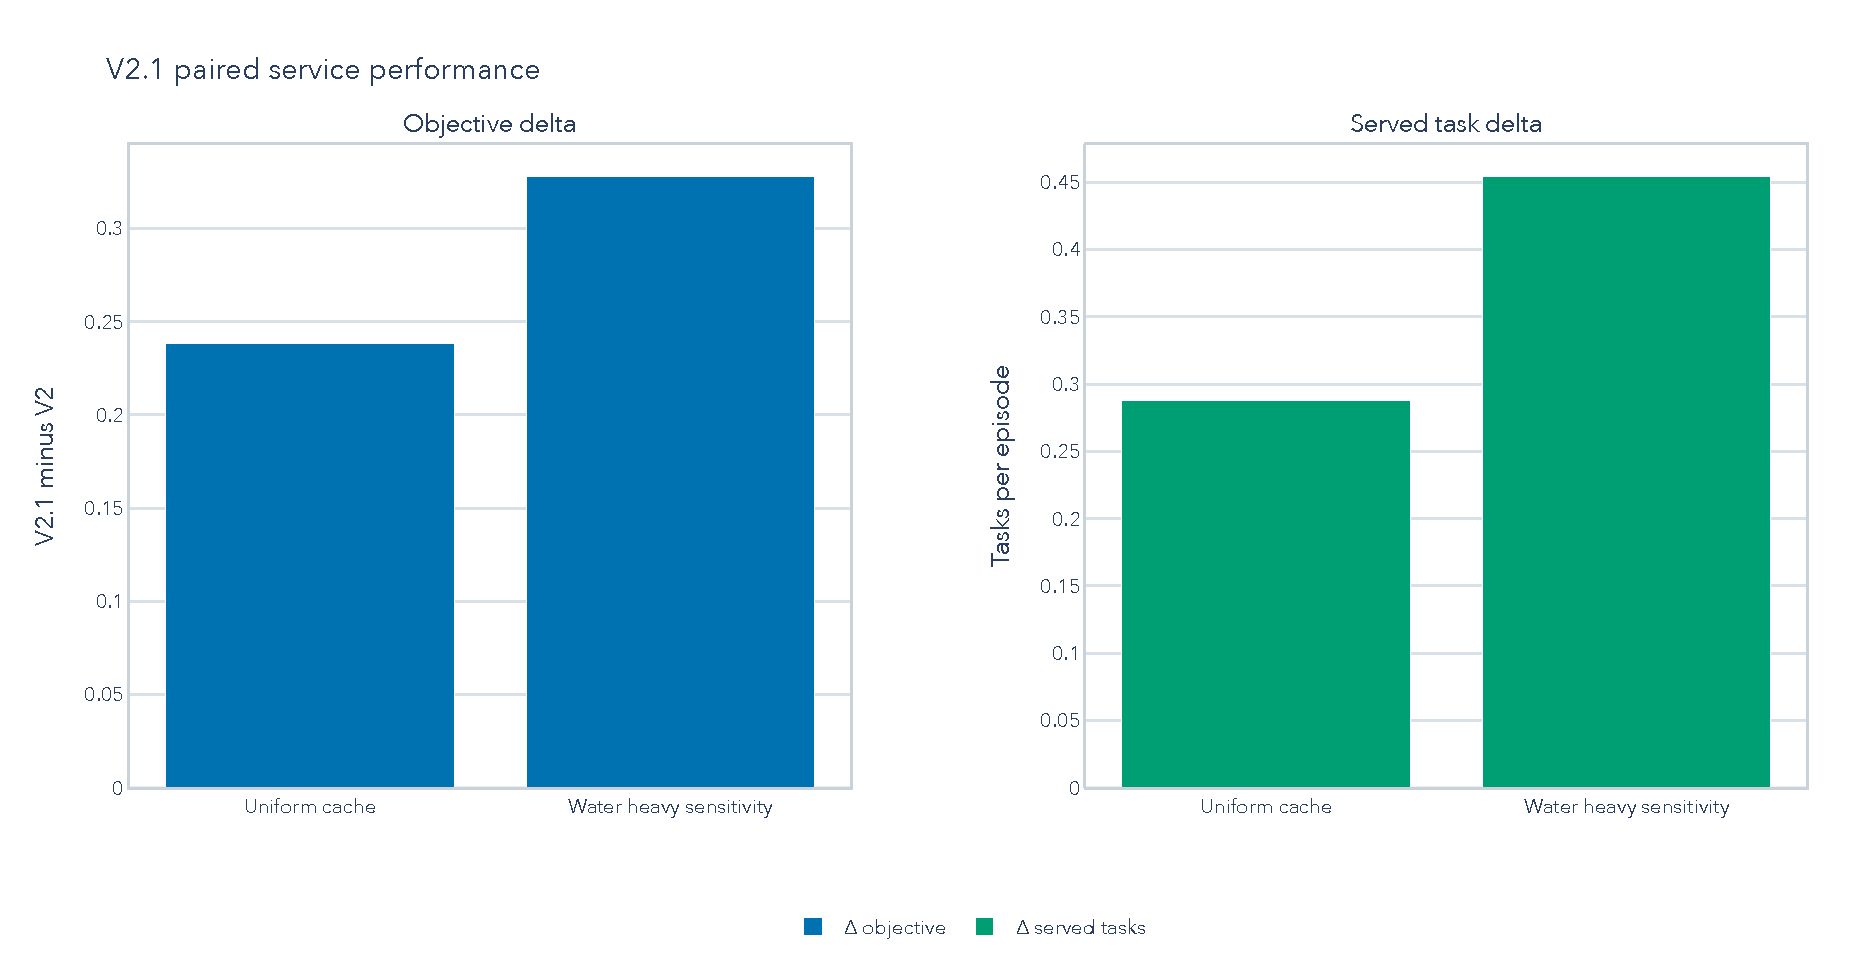
\includegraphics[width=0.98\textwidth]{../assets/v2_1/v2_1_paired_performance.pdf}\caption{V2.1 paired objective এবং served task delta।}\end{figure}
\section{Cache activity এবং environment sensitivity}
\begin{figure}[htbp]\centering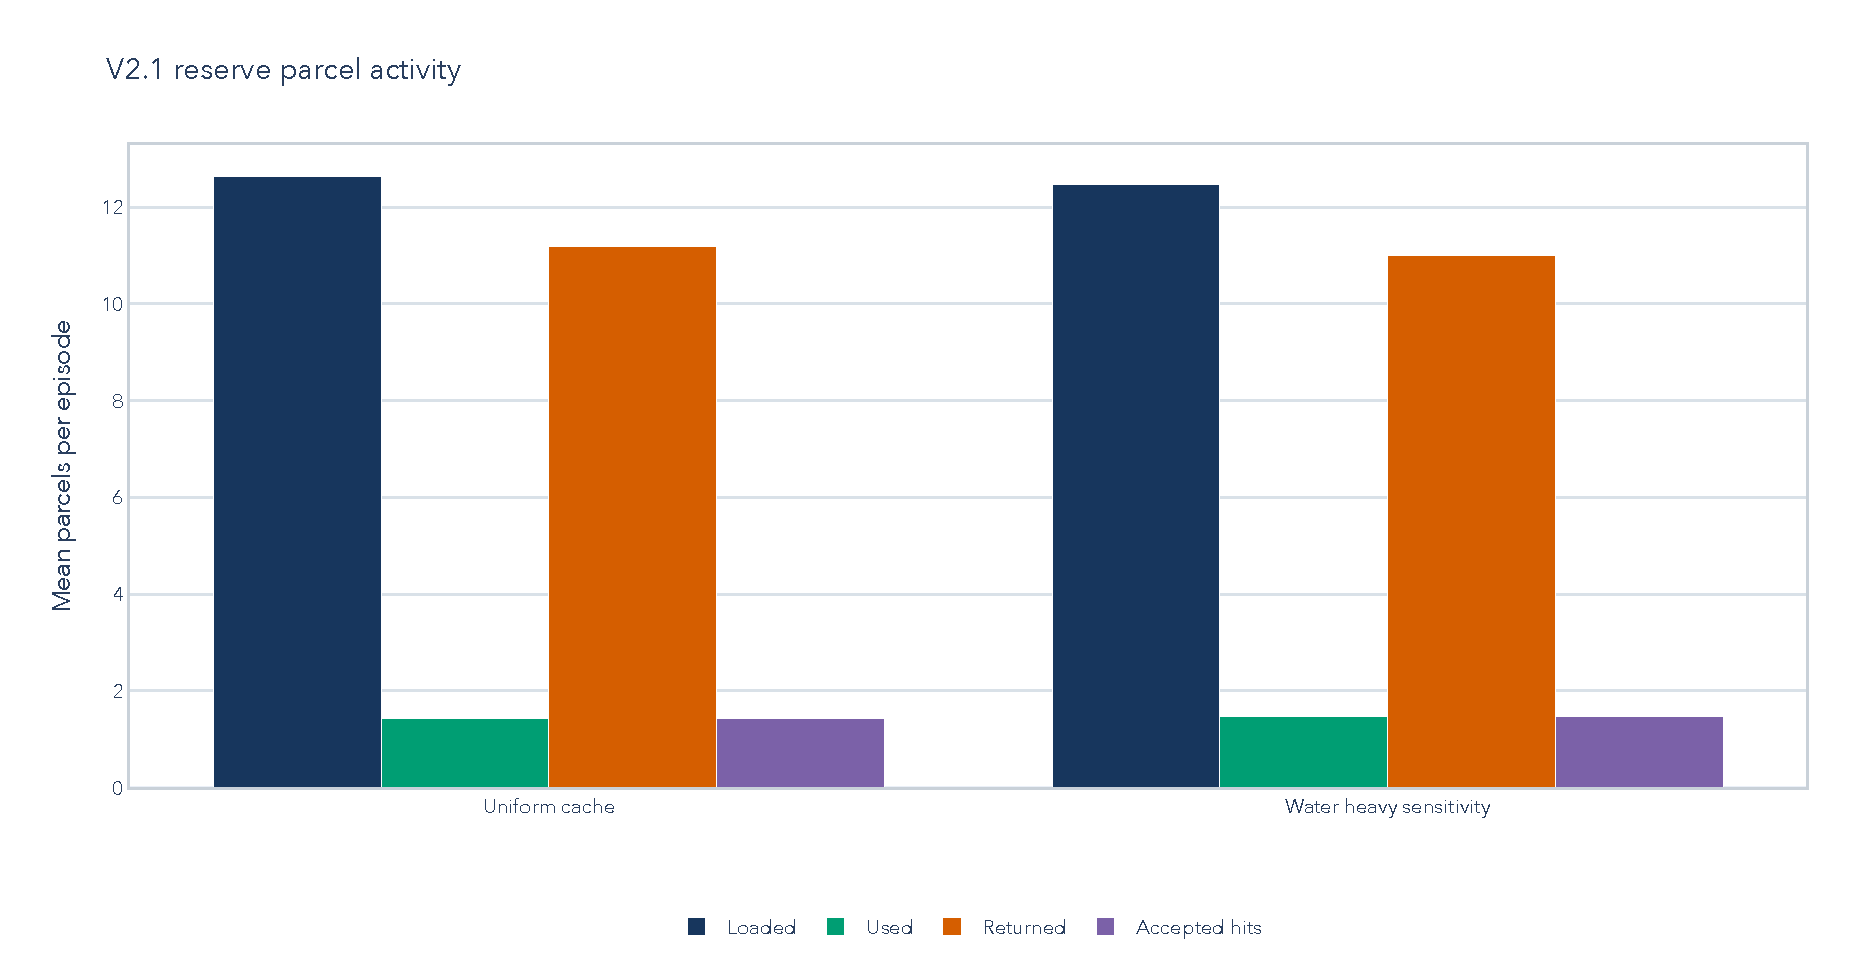
\includegraphics[width=0.98\textwidth]{../assets/v2_1/v2_1_cache_activity.pdf}\caption{Reserve parcel load, use, return এবং accepted hit।}\end{figure}
\begin{figure}[htbp]\centering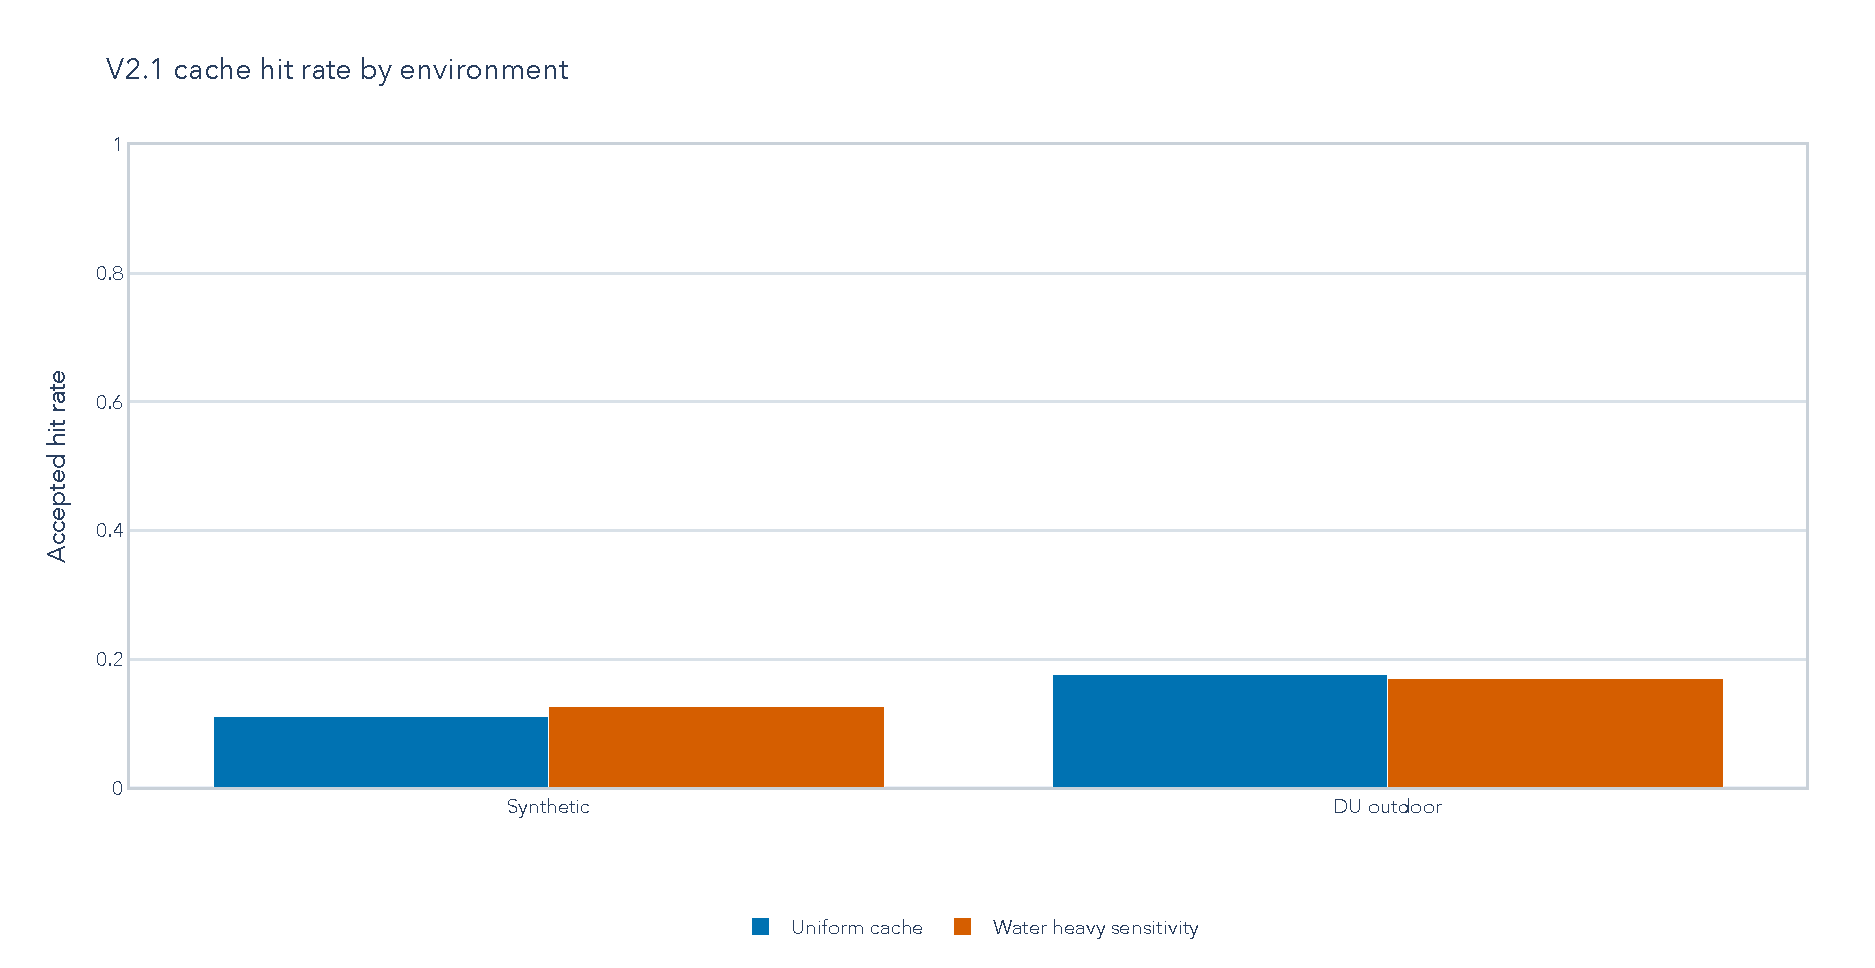
\includegraphics[width=0.98\textwidth]{../assets/v2_1/v2_1_hit_rate_environment.pdf}\caption{Environment অনুযায়ী cache hit rate।}\end{figure}
\begin{figure}[htbp]\centering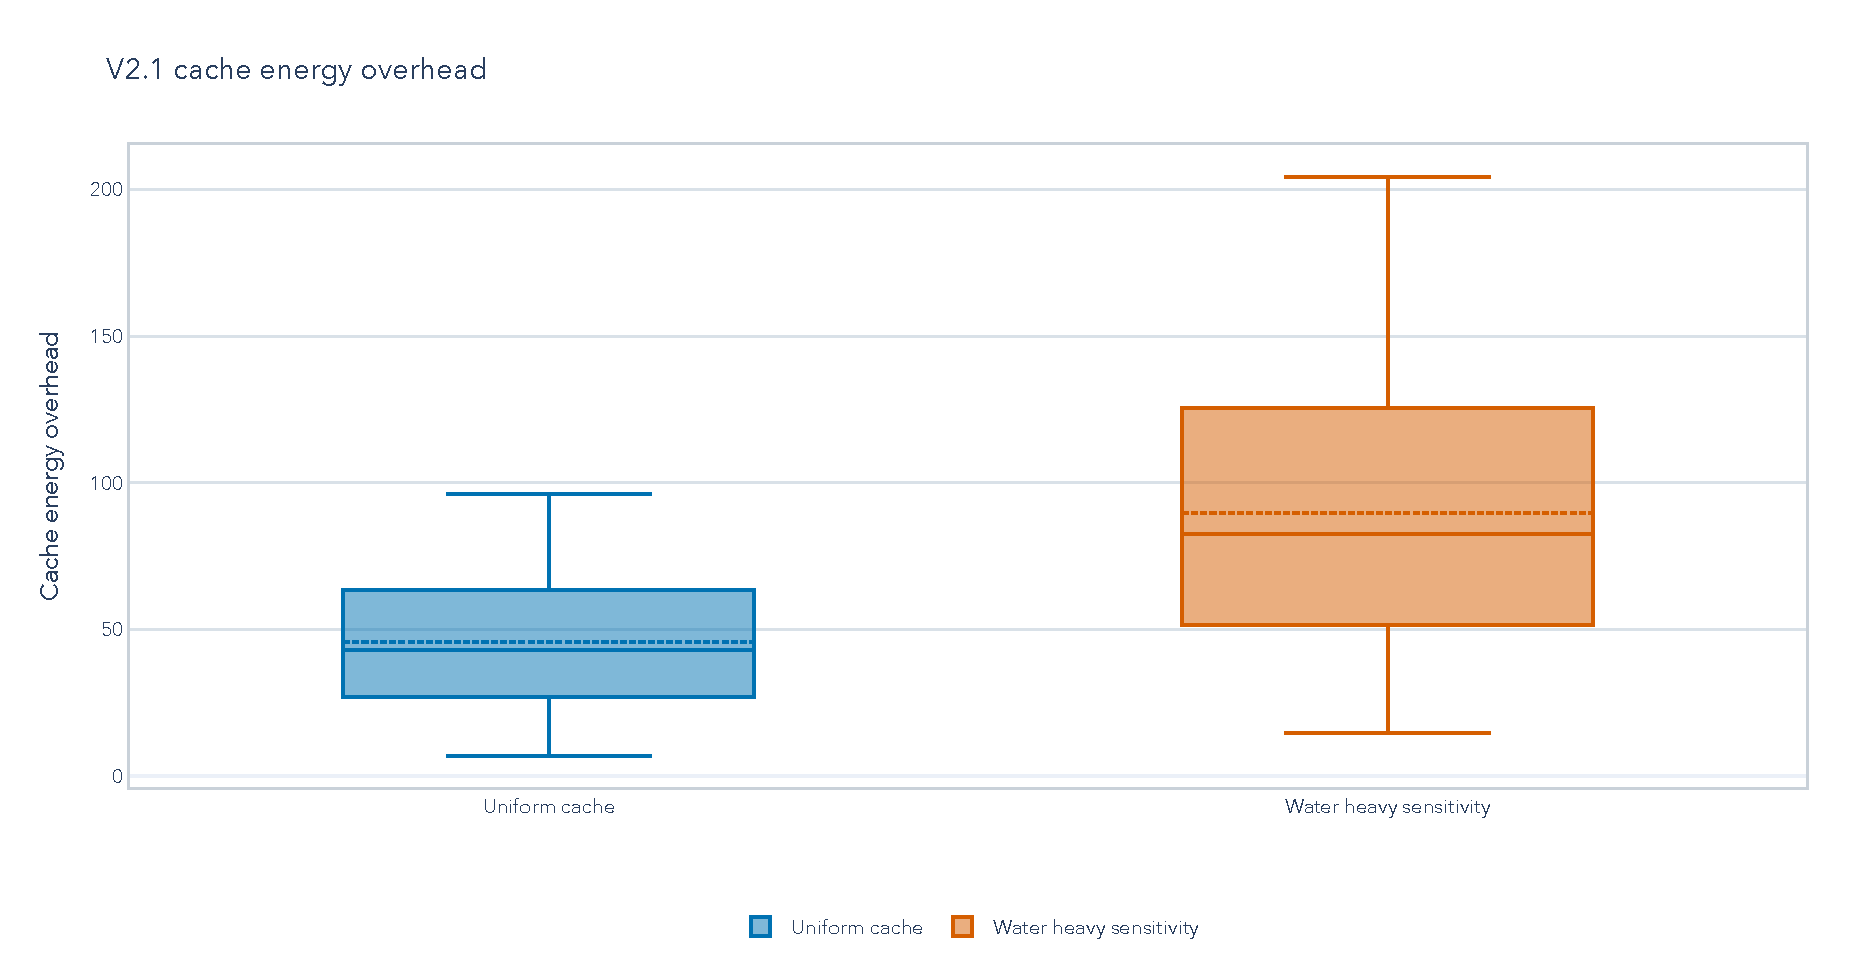
\includegraphics[width=0.98\textwidth]{../assets/v2_1/v2_1_energy_overhead.pdf}\caption{Cache energy overhead distribution।}\end{figure}
\begin{landscape}
\scriptsize
\begin{longtable}{@{}llrlrrrrrr@{}}
\caption{Environment, task load, fleet এবং policy অনুযায়ী সম্পূর্ণ V2.1 matrix summary।}\\
\toprule Environment & Task & UAV & Variant & Objective & Served & Delivery & Energy & Hit rate & Overhead\\\midrule
\endfirsthead
\toprule Environment & Task & UAV & Variant & Objective & Served & Delivery & Energy & Hit rate & Overhead\\\midrule
\endhead
DU outdoor & 30 & 3 & V2 control & 5.54 ± 1.11 & 9.10 ± 2.33 & 25.3\% & 2863.48 ± 223.88 & 0.0\% & 0.00 ± 0.00 \\
DU outdoor & 30 & 3 & Uniform cache & 5.73 ± 1.13 & 9.00 ± 2.00 & 26.0\% & 2922.77 ± 204.75 & 19.2\% & 25.33 ± 5.30 \\
DU outdoor & 30 & 3 & Water heavy sensitivity & 5.89 ± 1.05 & 9.70 ± 2.00 & 27.0\% & 2961.20 ± 257.12 & 12.1\% & 53.81 ± 16.16 \\
DU outdoor & 30 & 5 & V2 control & 7.80 ± 1.42 & 13.80 ± 3.36 & 39.9\% & 4616.14 ± 312.52 & 0.0\% & 0.00 ± 0.00 \\
DU outdoor & 30 & 5 & Uniform cache & 8.29 ± 1.44 & 14.30 ± 3.20 & 41.4\% & 4673.24 ± 281.94 & 17.0\% & 41.82 ± 9.83 \\
DU outdoor & 30 & 5 & Water heavy sensitivity & 8.34 ± 1.55 & 14.50 ± 3.54 & 43.4\% & 4696.47 ± 328.31 & 17.5\% & 80.49 ± 22.33 \\
DU outdoor & 30 & 8 & V2 control & 10.15 ± 1.69 & 19.20 ± 3.49 & 59.7\% & 6775.10 ± 391.17 & 0.0\% & 0.00 ± 0.00 \\
DU outdoor & 30 & 8 & Uniform cache & 10.41 ± 1.61 & 19.60 ± 3.72 & 61.4\% & 6808.41 ± 455.13 & 31.0\% & 64.59 ± 6.76 \\
DU outdoor & 30 & 8 & Water heavy sensitivity & 10.18 ± 1.78 & 19.10 ± 3.90 & 59.1\% & 6768.38 ± 463.68 & 16.1\% & 130.35 ± 16.61 \\
DU outdoor & 30 & 10 & V2 control & 10.85 ± 1.53 & 20.80 ± 3.12 & 65.7\% & 7700.52 ± 574.49 & 0.0\% & 0.00 ± 0.00 \\
DU outdoor & 30 & 10 & Uniform cache & 10.95 ± 1.50 & 20.80 ± 3.16 & 66.1\% & 7755.53 ± 572.91 & 16.8\% & 81.87 ± 8.83 \\
DU outdoor & 30 & 10 & Water heavy sensitivity & 10.86 ± 1.52 & 20.70 ± 3.02 & 65.3\% & 7787.81 ± 566.99 & 20.8\% & 162.59 ± 17.26 \\
DU outdoor & 60 & 3 & V2 control & 7.01 ± 1.19 & 10.10 ± 1.66 & 13.6\% & 3027.15 ± 216.04 & 0.0\% & 0.00 ± 0.00 \\
DU outdoor & 60 & 3 & Uniform cache & 6.86 ± 0.97 & 9.80 ± 1.32 & 13.8\% & 3016.09 ± 270.92 & 12.9\% & 26.15 ± 4.54 \\
DU outdoor & 60 & 3 & Water heavy sensitivity & 7.01 ± 1.03 & 10.00 ± 1.49 & 13.6\% & 3070.78 ± 194.24 & 14.5\% & 52.00 ± 9.95 \\
DU outdoor & 60 & 5 & V2 control & 9.85 ± 1.41 & 14.90 ± 1.97 & 20.7\% & 4886.49 ± 234.63 & 0.0\% & 0.00 ± 0.00 \\
DU outdoor & 60 & 5 & Uniform cache & 10.03 ± 1.51 & 15.10 ± 2.08 & 22.6\% & 5002.73 ± 188.73 & 18.3\% & 45.57 ± 8.91 \\
DU outdoor & 60 & 5 & Water heavy sensitivity & 9.76 ± 1.65 & 14.60 ± 2.17 & 21.8\% & 4744.61 ± 301.42 & 14.6\% & 76.92 ± 17.43 \\
DU outdoor & 60 & 8 & V2 control & 13.79 ± 1.87 & 22.40 ± 2.59 & 34.3\% & 7548.30 ± 510.66 & 0.0\% & 0.00 ± 0.00 \\
DU outdoor & 60 & 8 & Uniform cache & 13.56 ± 2.14 & 21.90 ± 3.00 & 34.2\% & 7533.59 ± 343.52 & 15.7\% & 67.95 ± 9.99 \\
DU outdoor & 60 & 8 & Water heavy sensitivity & 14.40 ± 2.38 & 23.30 ± 3.53 & 36.3\% & 7789.55 ± 383.07 & 15.0\% & 128.25 ± 28.14 \\
DU outdoor & 60 & 10 & V2 control & 15.85 ± 2.80 & 26.50 ± 4.48 & 41.8\% & 9270.10 ± 512.47 & 0.0\% & 0.00 ± 0.00 \\
DU outdoor & 60 & 10 & Uniform cache & 15.77 ± 2.79 & 26.50 ± 4.30 & 42.4\% & 9210.35 ± 627.87 & 18.6\% & 80.46 ± 9.47 \\
DU outdoor & 60 & 10 & Water heavy sensitivity & 16.56 ± 2.48 & 27.90 ± 4.09 & 44.8\% & 9516.09 ± 673.24 & 19.4\% & 159.36 ± 21.68 \\
DU outdoor & 90 & 3 & V2 control & 6.77 ± 1.50 & 9.40 ± 1.96 & 8.4\% & 2962.64 ± 230.76 & 0.0\% & 0.00 ± 0.00 \\
DU outdoor & 90 & 3 & Uniform cache & 7.23 ± 1.42 & 9.90 ± 1.79 & 9.1\% & 3125.02 ± 222.61 & 13.2\% & 27.36 ± 4.71 \\
DU outdoor & 90 & 3 & Water heavy sensitivity & 6.93 ± 1.36 & 9.60 ± 1.65 & 9.3\% & 2965.24 ± 282.12 & 25.0\% & 54.76 ± 8.40 \\
DU outdoor & 90 & 5 & V2 control & 10.39 ± 2.50 & 14.80 ± 3.12 & 14.0\% & 4748.06 ± 275.69 & 0.0\% & 0.00 ± 0.00 \\
DU outdoor & 90 & 5 & Uniform cache & 10.76 ± 2.21 & 15.00 ± 2.67 & 15.0\% & 4860.48 ± 232.78 & 12.5\% & 44.37 ± 7.75 \\
DU outdoor & 90 & 5 & Water heavy sensitivity & 11.07 ± 2.05 & 15.90 ± 2.18 & 15.8\% & 4905.60 ± 237.10 & 15.2\% & 83.34 ± 21.91 \\
DU outdoor & 90 & 8 & V2 control & 15.10 ± 2.94 & 22.60 ± 3.69 & 22.6\% & 7620.26 ± 381.34 & 0.0\% & 0.00 ± 0.00 \\
DU outdoor & 90 & 8 & Uniform cache & 15.73 ± 2.44 & 23.30 ± 3.27 & 24.0\% & 7795.50 ± 457.83 & 17.4\% & 69.94 ± 8.54 \\
DU outdoor & 90 & 8 & Water heavy sensitivity & 15.85 ± 3.12 & 23.50 ± 3.95 & 24.2\% & 7738.56 ± 351.28 & 15.0\% & 131.39 ± 25.03 \\
DU outdoor & 90 & 10 & V2 control & 17.90 ± 3.14 & 27.40 ± 4.38 & 28.3\% & 9396.49 ± 530.71 & 0.0\% & 0.00 ± 0.00 \\
DU outdoor & 90 & 10 & Uniform cache & 18.78 ± 2.99 & 28.90 ± 4.23 & 30.9\% & 9614.24 ± 388.53 & 18.0\% & 83.83 ± 10.25 \\
DU outdoor & 90 & 10 & Water heavy sensitivity & 18.38 ± 3.15 & 28.10 ± 4.53 & 29.4\% & 9379.10 ± 513.60 & 18.4\% & 170.95 ± 28.77 \\
Synthetic & 30 & 3 & V2 control & 12.26 ± 1.35 & 21.00 ± 2.16 & 65.5\% & 2749.05 ± 186.38 & 0.0\% & 0.00 ± 0.00 \\
Synthetic & 30 & 3 & Uniform cache & 12.38 ± 1.29 & 21.20 ± 2.04 & 66.2\% & 2763.38 ± 187.52 & 7.4\% & 14.05 ± 4.28 \\
Synthetic & 30 & 3 & Water heavy sensitivity & 12.47 ± 1.35 & 21.10 ± 2.18 & 66.3\% & 2751.32 ± 189.08 & 13.6\% & 25.71 ± 7.74 \\
Synthetic & 30 & 5 & V2 control & 15.30 ± 0.98 & 27.00 ± 1.56 & 89.0\% & 4080.53 ± 284.09 & 0.0\% & 0.00 ± 0.00 \\
Synthetic & 30 & 5 & Uniform cache & 15.16 ± 0.98 & 26.70 ± 1.34 & 87.3\% & 4093.29 ± 273.96 & 8.6\% & 33.29 ± 5.99 \\
Synthetic & 30 & 5 & Water heavy sensitivity & 15.37 ± 0.98 & 27.10 ± 1.45 & 89.4\% & 4164.14 ± 324.09 & 12.9\% & 67.24 ± 14.75 \\
Synthetic & 30 & 8 & V2 control & 16.28 ± 1.11 & 27.50 ± 1.43 & 90.9\% & 5003.03 ± 490.94 & 0.0\% & 0.00 ± 0.00 \\
Synthetic & 30 & 8 & Uniform cache & 16.28 ± 1.11 & 27.50 ± 1.43 & 90.9\% & 5061.38 ± 526.72 & 23.3\% & 56.33 ± 8.49 \\
Synthetic & 30 & 8 & Water heavy sensitivity & 16.29 ± 1.09 & 27.50 ± 1.43 & 90.9\% & 5114.90 ± 507.46 & 5.0\% & 113.07 ± 16.67 \\
Synthetic & 30 & 10 & V2 control & 16.44 ± 1.12 & 27.50 ± 1.43 & 90.9\% & 5209.87 ± 552.00 & 0.0\% & 0.00 ± 0.00 \\
Synthetic & 30 & 10 & Uniform cache & 16.44 ± 1.12 & 27.50 ± 1.43 & 90.9\% & 5271.93 ± 559.37 & 0.0\% & 62.06 ± 7.44 \\
Synthetic & 30 & 10 & Water heavy sensitivity & 16.44 ± 1.12 & 27.50 ± 1.43 & 90.9\% & 5333.99 ± 566.75 & 0.0\% & 124.12 ± 14.88 \\
Synthetic & 60 & 3 & V2 control & 15.54 ± 1.62 & 22.60 ± 2.72 & 33.5\% & 2819.10 ± 133.40 & 0.0\% & 0.00 ± 0.00 \\
Synthetic & 60 & 3 & Uniform cache & 15.44 ± 1.65 & 22.10 ± 2.64 & 33.0\% & 2816.79 ± 88.98 & 10.6\% & 15.68 ± 6.79 \\
Synthetic & 60 & 3 & Water heavy sensitivity & 15.50 ± 1.30 & 22.50 ± 2.07 & 33.9\% & 2863.78 ± 126.32 & 10.4\% & 29.38 ± 8.76 \\
Synthetic & 60 & 5 & V2 control & 22.47 ± 1.92 & 34.90 ± 3.98 & 54.6\% & 4547.61 ± 225.19 & 0.0\% & 0.00 ± 0.00 \\
Synthetic & 60 & 5 & Uniform cache & 22.46 ± 1.97 & 34.40 ± 3.78 & 53.7\% & 4534.45 ± 193.67 & 9.3\% & 25.37 ± 2.10 \\
Synthetic & 60 & 5 & Water heavy sensitivity & 22.61 ± 1.83 & 34.70 ± 3.27 & 54.4\% & 4639.60 ± 214.22 & 16.6\% & 52.53 ± 11.51 \\
Synthetic & 60 & 8 & V2 control & 29.51 ± 2.47 & 50.20 ± 5.55 & 81.6\% & 7001.95 ± 249.08 & 0.0\% & 0.00 ± 0.00 \\
Synthetic & 60 & 8 & Uniform cache & 29.78 ± 2.49 & 50.50 ± 4.74 & 82.1\% & 7002.92 ± 344.91 & 15.7\% & 41.45 ± 8.59 \\
Synthetic & 60 & 8 & Water heavy sensitivity & 29.85 ± 2.37 & 50.90 ± 4.65 & 83.0\% & 7127.86 ± 338.59 & 15.9\% & 82.12 ± 13.58 \\
Synthetic & 60 & 10 & V2 control & 31.67 ± 1.87 & 54.30 ± 2.83 & 89.4\% & 8068.17 ± 540.13 & 0.0\% & 0.00 ± 0.00 \\
Synthetic & 60 & 10 & Uniform cache & 31.80 ± 1.69 & 54.60 ± 2.32 & 90.1\% & 8169.13 ± 583.65 & 10.6\% & 61.12 ± 8.83 \\
Synthetic & 60 & 10 & Water heavy sensitivity & 31.87 ± 1.65 & 54.80 ± 1.99 & 90.4\% & 8306.50 ± 653.75 & 20.3\% & 124.17 ± 18.99 \\
Synthetic & 90 & 3 & V2 control & 16.61 ± 1.60 & 22.70 ± 2.16 & 21.8\% & 2814.47 ± 115.30 & 0.0\% & 0.00 ± 0.00 \\
Synthetic & 90 & 3 & Uniform cache & 17.10 ± 1.49 & 23.10 ± 1.91 & 22.8\% & 2885.27 ± 92.69 & 10.5\% & 15.59 ± 3.71 \\
Synthetic & 90 & 3 & Water heavy sensitivity & 17.41 ± 1.60 & 23.80 ± 2.25 & 23.1\% & 2903.20 ± 92.92 & 14.4\% & 25.01 ± 6.83 \\
Synthetic & 90 & 5 & V2 control & 25.36 ± 2.45 & 36.50 ± 3.66 & 35.8\% & 4699.38 ± 157.17 & 0.0\% & 0.00 ± 0.00 \\
Synthetic & 90 & 5 & Uniform cache & 25.77 ± 2.14 & 37.30 ± 3.13 & 37.4\% & 4803.85 ± 166.39 & 10.1\% & 24.53 ± 6.87 \\
Synthetic & 90 & 5 & Water heavy sensitivity & 26.04 ± 2.15 & 37.40 ± 3.24 & 37.0\% & 4808.84 ± 98.43 & 13.1\% & 46.33 ± 10.29 \\
Synthetic & 90 & 8 & V2 control & 35.30 ± 3.12 & 55.30 ± 5.38 & 57.7\% & 7364.18 ± 246.65 & 0.0\% & 0.00 ± 0.00 \\
Synthetic & 90 & 8 & Uniform cache & 35.97 ± 3.06 & 56.40 ± 4.93 & 59.2\% & 7426.48 ± 216.50 & 11.6\% & 41.14 ± 8.13 \\
Synthetic & 90 & 8 & Water heavy sensitivity & 35.72 ± 2.97 & 55.60 ± 4.97 & 58.5\% & 7453.48 ± 230.75 & 14.9\% & 76.37 ± 18.88 \\
Synthetic & 90 & 10 & V2 control & 40.55 ± 3.31 & 66.80 ± 6.00 & 71.2\% & 8962.54 ± 239.81 & 0.0\% & 0.00 ± 0.00 \\
Synthetic & 90 & 10 & Uniform cache & 41.29 ± 2.93 & 68.80 ± 4.59 & 74.3\% & 9160.76 ± 266.98 & 14.3\% & 48.48 ± 8.00 \\
Synthetic & 90 & 10 & Water heavy sensitivity & 41.34 ± 2.93 & 68.40 ± 4.81 & 73.8\% & 9123.56 ± 270.96 & 14.3\% & 99.98 ± 18.62 \\
\bottomrule
\end{longtable}
\end{landscape}
\section{Decision এবং limitations}
প্রথম full matrix one-slot cache policy retain করার পক্ষে evidence দিয়েছে। দ্বিতীয় slot এবং adaptive prior আপাতত defer করা হয়েছে, কারণ অধিকাংশ loaded parcel unused অবস্থায় return করেছে এবং water-heavy sensitivity cache energy overhead বাড়িয়েছে। Item prior field-calibrated probability নয়। Matrix bounded planner settings ব্যবহার করেছে এবং unrestricted optimality claim করে না।
\section{Evidence এবং reproducibility}
Raw metrics, decision traces, summary CSV এবং manifest Simulation results folder-এ সংরক্ষিত। V2.1 code আলাদা v2\_1 namespace-এ এবং এই report-এর editable source V2.1 report folder-এ রাখা হয়েছে।
\end{document}
